%%%%%%%%%%%%%%%%%%%%%%%%%%%%%%%%%%%%%%%%%%%%%%%%%%%%%%%%%%%%%%%%%%%%%%%%
%    INSTITUTE OF PHYSICS PUBLISHING                                   %
%                                                                      %
%   `Preparing an article for publication in an Institute of Physics   %
%    Publishing journal using LaTeX'                                   %
%                                                                      %
%    LaTeX source code `ioplau2e.tex' used to generate `author         %
%    guidelines', the documentation explaining and demonstrating use   %
%    of the Institute of Physics Publishing LaTeX preprint files       %
%    `iopart.cls, iopart12.clo and iopart10.clo'.                      %
%                                                                      %
%    `ioplau2e.tex' itself uses LaTeX with `iopart.cls'                %
%                                                                      %
%%%%%%%%%%%%%%%%%%%%%%%%%%%%%%%%%%
%
%
% First we have a character check
%
% ! exclamation mark    " double quote
% # hash                ` opening quote (grave)
% & ampersand           ' closing quote (acute)
% $ dollar              % percent
% ( open parenthesis    ) close paren.
% - hyphen              = equals sign
% | vertical bar        ~ tilde
% @ at sign             _ underscore
% { open curly brace    } close curly
% [ open square         ] close square bracket
% + plus sign           ; semi-colon
% * asterisk            : colon
% < open angle bracket  > close angle
% , comma               . full stop
% ? question mark       / forward slash
% \ backslash           ^ circumflex
%
% ABCDEFGHIJKLMNOPQRSTUVWXYZ
% abcdefghijklmnopqrstuvwxyz
% 1234567890
%
%%%%%%%%%%%%%%%%%%%%%%%%%%%%%%%%%%%%%%%%%%%%%%%%%%%%%%%%%%%%%%%%%%%
%
\documentclass[12pt,a4paper,final]{iopart}
\newcommand{\gguide}{{\it Preparing graphics for IOP journals}}
%Uncomment next line if AMS fonts required
\usepackage{iopams}
\usepackage{graphicx}
\usepackage[breaklinks=true,colorlinks=true,linkcolor=blue,urlcolor=blue,citecolor=blue]{hyperref}
%\usepackage{amsmath,amssymb,amsthm,amscd}
%\usepackage{natbib}

\usepackage[all]{xy}
\newcommand{\eq}{\mbox{eq}}
\newcommand{\dt}{\mathit{dt}}
\newcommand{\bbM}{\mathbb M}
\newcommand{\bt}{\pmb\theta}
\newcommand{\Bt}{\pmb\Theta}
\newcommand{\vc}[1]{{\bf #1 }}


\begin{document}

\title[Parameter inference with stochastic models]{Parameter Inference for a Simple Stochastic Hydrological Model}

\author[cor1]{Carlo Albert}%$^{1,2}$
\address{Eawag, Swiss Federal Institute of Aquatic Science and Technology, 8600 Dübendorf, Switzerland}
%\address{$^2$Address Two, Neverland}
\ead{carlo.albert@eawag.ch}

\author{Simone Ulzega}
\address{Eawag, Swiss Federal Institute of Aquatic Science and Technology, 8600 Dübendorf, Switzerland}
\ead{simone.ulzega@eawag.ch}

%\author[cor1]{Author Three}
%\address{Address Four, Neverland}
%\eads{\mailto{author.three@mail.com}, \mailto{author.three@gmail.com}}


\begin{abstract}
\textbf{[TO BE WRITTEN]} This document describes the  preparation of an article using \LaTeXe\ and \verb"iopart.cls" (the IOP \LaTeXe\ preprint class file).
This class file is designed to help
authors produce preprints in a form suitable for submission to any of the
journals published by IOP Publishing.
Authors submitting to any IOP journal, i.e.\
both single- and double-column ones, should follow the guidelines set out here.
On acceptance, their TeX code will be converted to
the appropriate format for the journal concerned.

\end{abstract}

%Uncomment for PACS numbers title message
\pacs{00.00, 20.00, 42.10}
% Keywords required only for MST, PB, PMB, PM, JOA, JOB?
\vspace{2pc}
\noindent{\it Keywords}: Article preparation, IOP journals
% Uncomment for Submitted to journal title message
\submitto{\NJP}
% Comment out if separate title page not required
%\maketitle

\section{Introduction}

In this paper, we study the feasibility of a full Bayesian inference, for simple conceptual rainfall-runoff models with scale-invariant noise.
We start with a single linear reservoir and describe the dynamics of its water content, $S(t)$, by means of the stochastic differential equation
\begin{equation}\label{sde}
\dot{S}(t) = r(t) - \frac{1}{K}\left(1+\frac{\gamma}{2}\right) S(t)
+
\sqrt{\frac{\gamma}{K}} S(t){\eta}(t)\,,
\end{equation}
where $r(t)$ describes the rain input and $\eta(t)$ denotes white noise, i.e.,
\begin{equation}\label{whitenoise}
\langle\eta(t)\eta(t')\rangle = \delta(t-t')\,.
\end{equation}
Due to the state-dependence of the noise term, Eq.~(\ref{sde}) is ill-defined unless we specify the discretization convention.
For computational reasons, we work with the {\em Stratonovich} convention.
Our parametrization is such that, for constant rain input $r(t)=r_0$ and in the long-time limit, the mean of $S$ converges to the equilibrium solution of the unperturbed ($\gamma=0$) system, $S_{\eq}=Kr_0$ (see below).

The scale-invariance of the noise term renders the noise parameter $\gamma$ dimensionless.
Before we proceed, we replace the state variable $S(t)$ and parameter $K$ by dimensionless quantities $q(t)$ and $\beta$, respectively, by means of the transformations
\begin{equation}
  \beta=\sqrt{\frac{T\gamma}{K}}\,,\quad
  S(t)=\frac{T\gamma r(t)}{\beta^2}e^{\beta q(t)}\,.
\end{equation}
W.r.t. these new  variables and parameters, the model equation (\ref{sde}) becomes
\begin{equation}
  \dot q(t)
  =
  \frac{\beta}{T\gamma}e^{-\beta q(t)}
  -
  \frac{1}{T}\rho(t)
  +
  \frac{1}{\sqrt{T}}\eta(t)\,,
\end{equation}
with
\begin{equation}
  \rho(t)
  =
  \frac{T}{\beta}\frac{d}{dt}\ln r(t)
  +
  \frac{(2+\gamma)\beta}{2\gamma}\,.
\end{equation}

According to Ref.~\cite{lau_2007}, the probability $P(q_1,T|q_0,0)$ of finding the system in a state $q$ at time $t = T$ given that it was in an initial state $q_0$ at time $t = 0$, can be expressed in the form of a path integral as
\begin{equation}\label{pathint}
P(q_1,T|q_0,0)
=
\frac{1}{Z}
\int
e^{-{\mathcal S}[q,\dot q]}
\delta(q(T)-q_1)
\delta(q(0)-q_0)
\mathcal{D}q \,,
\end{equation}
where the integral extends over all paths $q:[0,T]\rightarrow \mathbb R$.
The path-measure $\mathcal Dq$ is formally written as an infinite product
\begin{equation}\label{pathmeasure_q}
{\mathcal Dq}
=
\prod_{t}
dq(t)\,.
\end{equation}
The {\em action} is a functional on the space of paths and reads as
\begin{equation}\label{action1}
{\mathcal S}[{q},\dot q]
=
\frac{1}{T}
\int_0^T \dt \left\{
\frac{1}{2}
\left(
    T\dot q(t)
    +
    \rho(t)
    -
    \frac{\beta}{\gamma}e^{-\beta q(t)}\right)^2
    -
    \frac{\beta^2}{2\gamma}e^{-\beta q(t)}
\right\} \,.
\end{equation}
Note that the action includes the Jacobian that arises when changing coordinates from ${\eta(t)}$ to $q(t)$.

We introduce the time-dependent {\em Hamiltonian}
\begin{equation}\label{H}
  \mathcal{H}(q,t)
  =
  \frac{1}{\gamma}e^{-\beta q}+q\rho(t)\,,
\end{equation}
and rewrite the action~(\ref{action1}) as,
\begin{eqnarray}\label{action}
{\mathcal S}[{q},\dot q] \nonumber
\\
= \frac{1}{T}
\int_0^T dt\left\{
    \frac{1}{2}
    T^2\dot q^2(t) +
    \frac{1}{2}
    \left(\rho(t)-\frac{\beta}{\gamma}e^{-\beta q(t)}\right)^2 -
    T\frac{\partial \mathcal{H}(q,t)}{\partial t} -
    \frac{\beta^2}{2\gamma}e^{-\beta q(t)}
     %\frac{(2+\gamma)\beta^2}{4\gamma}
\right\} \nonumber
\\
+ \mathcal{H}(q(T),T) - \mathcal{H}(q(0),0) \nonumber
\\
= \frac{1}{T}
\int_0^T dt\left\{
    \frac{1}{2}
    T^2\dot q^2(t) +
    \frac{1}{2}
    \left(\rho(t)-\frac{\beta}{\gamma}e^{-\beta q(t)}\right)^2 -
    Tq(t)\dot\rho(t) -
     \frac{\beta^2}{2\gamma}e^{-\beta q(t)}
%    \frac{(2+\gamma)\beta^2}{4\gamma}
\right\}  \nonumber
\\
+
    \frac{1}{\gamma}e^{-\beta q(T)}+q(T)\rho(T)
   -\frac{1}{\gamma}e^{-\beta q(0)}-q(0)\rho(0)
\,.
\end{eqnarray}

Next, we calculate the equilibrium distribution $P_{\eq}(q) = \lim_{T\rightarrow\infty} P(q,T|q_0,0)$ in the simple case of a constant rain input $r(t)\equiv r_{0}$. Systems at thermal equilibrium must fulfill detailed balance, i.e.,
\begin{equation}\label{detailed_balance}
P(q_1 t_1 | q_0 t_0 ) P_{\eq}(q_0) = P(q_0 t_1 | q_1 t_0 ) P_{\eq}(q_1) \,.
\end{equation}
After plugging in (\ref{pathint}) and (\ref{action}), and using the transformation $q(t) \rightarrow q(-t)$, which maps paths from $q_0$ to $q_1$ to paths from $q_1$ to $q_0$, we get, since $\dot\rho(t)= 0$,
\begin{equation}\label{Peq}
  P_{\eq}(q)
  \propto
  e^{-2\mathcal{H}(q)}\,.
\end{equation}
Transforming back to the original variables, it turns out that $P_{\eq}(S)$ is described by an inverse gamma distribution with scale parameter $2Kr_{0}/\gamma$ and shape parameter $(2+\gamma)/\gamma$, i.e.,
\begin{equation}\label{inverse_gamma}
  P_{\eq}(S)
  \propto
  S^{-2(1+\gamma)/\gamma}e^{-2Kr_{0}/(\gamma S)}\,,
\end{equation}
whose mean equals the equilibrium solution of the unperturbed system ($\gamma=0$),
\begin{equation}
  \langle S\rangle_{\eq}=Kr_{0},
\end{equation}
and whose variance, for $\gamma< 2$, is given by
\begin{equation}
  \langle (S - \langle S\rangle_{\eq})^2\rangle_{\eq}
  =
  K^2r_{0}^2
  \frac{\gamma}{2-\gamma}\,.
\end{equation}
Note that the variance diverges, for $\gamma\geq 2$.
The power-law decay of the inverse gamma distribution is reminiscent of the scale-invariance of the error model.

Let us now consider two time-series of {\em observed} rain inputs and discharge outputs, $r_s=r(t_s)$ and $y_s=S(t_s)/K$, respectively, measured at times $0=t_1<t_2<\dots < t_{n+1}=T$.
For the measurement error model, we simply set
\begin{equation}\label{data}
  \ln\frac{y_s}{r_s}
  =
  \beta q_s
  +
  \sigma\epsilon_s\,,\quad s=1,\dots,n+1\,,
\end{equation}
where $\epsilon_s$ are uncorrelated standard normal random variables.

The goal is to infer the posterior parameter distribution, for the parameters $\bt=(\beta,\gamma)^T$, based on the measured time series $\vc r$ and $\vc y$.
For the time being we assume constant priors.
Then, the posterior reads as
\begin{equation}\label{posterior_pathint}
  f(\bt | \vc y, \vc r)
  \propto
  \int
  \exp\bigg[
    -{{\mathcal S}}[{q},\dot q]
    -\frac{1}{2}
    \sum_{s=1}^{n+1}
    \frac
    {(\ln(y_s/r_s)-{\beta q_s})^2}
    {\sigma^2}
    %-\ln(K\gamma)
  \bigg]
  {\mathcal Dq}
  \,.
\end{equation}
Since the integral on the r.h.s. of (\ref{posterior_pathint}) is very expensive to calculate, we will sample, simultaneously, parameter vectors $\bt$ and discretized system realizations $q(t)$ directly from an appropriate discretization of the kernel of (\ref{posterior_pathint}).
Since the associated distribution is very high dimensional and strongly correlated, we employ the method called {\em Hamiltonian Monte Carlo} (HMC) introduced by Ref.~\cite{duane_1987}.
This method interprets the exponent of the kernel of the posterior as the potential of a one-dimensional statistical mechanical system. Each degree of freedom, $q(t)$ and $\bt$ in our case, is paired with a conjugate variable, $p(t)$ and ${\pmb\pi}$, respectively, and the system is defined by the  Hamiltonian
\begin{equation}\label{Hamiltonian}
    \mathcal{H}_{\mbox{\tiny HMC}}(q,\bt; p,{\pmb\pi})
    =
    K( p,{\pmb\pi}) + V( q,\bt)\,,
\end{equation}
with
\begin{equation}\label{K}
   K( p,{\pmb\pi})
   =
   \int_0^T \frac{ p^2(t)}{2m(t)}dt
   + \sum_{\alpha=1}^2\frac{\pi_\alpha^2}{2m_\alpha}\,,
\end{equation}
where $V( q,\bt)$ is the negative logarithm of the kernel of (\ref{posterior_pathint}).
The posterior (\ref{posterior_pathint}) is expressed by the phase space path integral
\begin{equation}\label{phaseSpacePathInt}
    f(\bt | \vc y, \vc r)
  \propto
  \int
  e^{-\mathcal {H}_{\mbox{\tiny HMC}}(q,\bt; p,{\pmb\pi})}
  {\mathcal Dp}
  \wedge
  {\mathcal Dq}
  \wedge
  d{\pmb\pi}
  \,.
\end{equation}

The HMC method, which is a combination of the {\em Metropolis algorithm} of Ref.~\cite{metropolis_1953} and {\em molecular dynamics} methods \textbf{[ref?]}, iterates the following steps,
\begin{enumerate}
  \item
  Momenta are sampled from the Gaussian distribution defined by (\ref{K}).
  \item
  A volume-preserving and time-reversible solution to a discretization of Hamilton's equations is calculated numerically.
  \item
  The discretization error on the energy preservation due to the previous step is corrected by a Metropolis acceptance/rejection step.
\end{enumerate}
The last step is the standard Metropolis algorithm, while the first two steps allow us to make relatively large jumps in phase space while maintaining a relatively large acceptance rate.

Let us first write down the discretization of the path-integral (\ref{phaseSpacePathInt}).
Therefore, let us assume that the measurement time points $\left\{ y_s \right\}_{s=1,\dots, n+1}$ of the time series (\ref{data}) are equidistantly distributed on the time interval $[0,T]$, with $t_1=0$ and $t_{n+1}=T$.
Each interval between two consecutive data points is further partitioned into $j$ bins, such that we have a total of $nj+1=N>>1$ discretization points.
Path-integral (\ref{posterior_pathint}) is approximated by an ordinary integral, with the approximate path-measure
\begin{equation}
  \mathcal Dp\wedge\mathcal Dq
  \approx
  \prod_i dp_i\wedge dq_i
\end{equation}
and the discretized versions of $K( p,{\pmb\pi})$ and $V( q,\bt)$
\begin{eqnarray}
   K( p,{\pmb\pi}) \approx
   \sum_{i=1}^N
   \frac{ p_i^2}{2m_q}\Delta t
   +
   \sum_{\alpha=1}^2\frac{\pi_\alpha^2}{2m_\alpha}\,,\label{Kdisc}
   \\
   V(q,\bt) \approx \frac{\Delta t}{T} \sum_{i=2}^{N}
   \left\{ \frac{1}{2} T^2 \dot q_i^2 + \frac{1}{2}
     \left( \rho_i-\frac{\beta}{\gamma}e^{-\beta q_i} \right)^2 -
    \frac{\beta^2}{2\gamma} e^{-\beta q_i} - T q_i\dot\rho_i \right\}  \nonumber
  \\
  +
  \frac{1}{\gamma}
  e^{-\beta q_N}
  +
  q_N \rho_{N}
  -
  \frac{1}{\gamma}
  e^{-\beta q_1}
  -
  q_1 \rho_{1}
  \nonumber
  \\
  +
  \sum_{s=1}^{n+1}
  \frac{(\ln(y_s/r_{(s-1)j+1}) - {\beta q_{(s-1)j+1}})^2}{2\sigma^2}
  \label{Vdisc}
   \,,
\end{eqnarray}
with
\begin{equation}
  \dot q_i = \frac{q_i-q_{i-1}}{\Delta t}\,,
  %\quad
%  \bar q_i = \frac{q_i+q_{i-1}}{2}\,,
\end{equation}
and
\begin{equation}\label{rhodisc}
\rho_i = \frac{T}{\beta} \frac{\ln(r_{i}/r_{i-1})}{\Delta t}
+
\frac{(2+\gamma)\beta}{2\gamma}
\,,\quad
\dot\rho_i = \frac{\rho_i-\rho_{i-1}}{\Delta t}\,.
\end{equation}
Note that we've neglected terms of order $\mathcal O(N^{-1/2})$ in the action (\ref{Vdisc}) and that we've assumed $r_i$ to be the discretization of an at least twice differentiable interpolation of the input measurements.

For strongly varying rain input or high-frequency output data, $\Delta t$ needs to be chosen small. Thus, the harmonic part of the Hamiltonian becomes stiff and, consequently, the time-step of MD needs to be chosen small, which leads to slow convergence.
To solve this problem, we change coordinates, such that the harmonic part of the Hamiltonian becomes (partly) diagonal and the particle interaction moves to the potential.
One option would be to use the Fourier modes of ${\eta}(t)$ as configurational variables. Calculating the potential requires then an inversion of a Toeplitz matrix. This approach is interesting because, in our case, it allows for an approximate analytical integration of high-frequency modes as outlined in Ref.~\cite{doll_1985}.

We choose however another approach, the so-called \emph{staging} as described in Ref.~\cite{tuckerman_1992}, and diagonalize the harmonic part only in between the measurement points.
We first note that the Hamiltonian (\ref{Hamiltonian}) can be seen as the classical Hamiltonian of a polymer chain with harmonic bonds between neighbouring beads, described by the first harmonic term of $V(q,\bt)$, in an external field described by the other non-harmonic terms of $V(q,\bt)$.
Furthermore, the model parameters are viewed as additional degrees of freedom that couple with all other degrees of freedom.
Sampling system realizations, each defined by a set of coordinates $\left\{ q_i\right\}$ and parameters $\bt$, is equivalent to sampling states in the polymer dynamics.

The discretized harmonic part of the action is rewritten as
\begin{eqnarray}
  \sum_{i=2}^{N}
  \frac{T}{2\Delta t}
  (q_i-q_{i-1})^2 \nonumber
  \\ =
  \frac{T}{2}
  \sum_{s=1}^{n}\left\{
    \frac{(q_{(s-1)j+1} - q_{sj+1})^2}{j\Delta t}
    +
    \sum_{k=2}^j
    \frac{k}{(k-1)\Delta t}
    (q_{(s-1)j+k}-q^*_{(s-1)j+k})^2
  \right\}\,,\nonumber
  \\
\end{eqnarray}
with
\begin{equation}
  q^*_{(s-1)j+k}
  =
  \frac{(k-1)q_{(s-1)j+k+1} + q_{(s-1)j+1} }{k}
  \,.
\end{equation}
Following Ref.~\cite{tuckerman_1993} we apply the coordinate transformation
\begin{equation}
  u_{sj+1} = q_{sj+1}\,,\quad
  u_{sj+k} = q_{sj+k} - q^*_{sj+k}\,,
\end{equation}
with its inverse given by
\begin{equation}
  q_{sj+1} = u_{sj+1}\,,\quad
  q_{sj+k} = \sum_{l=k}^{j+1}\frac{k-1}{l-1}u_{sj+l}
  +\frac{j-k+1}{j}u_{sj+1}\,,
\end{equation}
or equivalently by the recursive relation
\begin{equation}
  q_{sj+k} = u_{sj+k} + \frac{k-1}{k} q_{sj+k+1}+ \frac{1}{k}u_{sj+1} \,.
\end{equation}


This transformation decouples fast degrees of freedom from slow ones and allows us to split the Hamiltonian $\mathcal{H}_{\mbox{\tiny HMC}}$ into components with different scaling behaviour in the potentially large numbers $n$ and $N$.
We write
\begin{equation}
  \mathcal{H}_{\mbox{\tiny HMC}}= \mathcal H_N+\mathcal H_n+\mathcal H_1\,,
\end{equation}
where
\begin{eqnarray}
  \mathcal H_N =
  \frac{1}{2}
  \sum_{s=1}^{n}
  \sum_{k=2}^j
  \left\{
    \frac{\Delta t}{m_q}p_{(s-1)j+k}^2
    +
    \frac{Tk}{\Delta t(k-1)}
    u_{(s-1)j+k}^2
  \right\}\,,\label{H_N}
  \\
  \mathcal H_n =
  \frac{1}{2}
  \sum_{s=1}^{n+1}
  \left\{
   \frac{\Delta t }{m_q}p_{(s-1)j+1}^2
    +
    \frac{(\ln(y_s/r_{(s-1)j+1}) - {\beta u_{(s-1)j+1}})^2}{\sigma^2}
   \right\} \nonumber
   \\
  +
  \frac{T}{2j\Delta t}
  \sum_{s=1}^{n}
    (u_{(s-1)j+1} - u_{sj+1})^2
   \,, \label{H_n} \\
  \mathcal H_1=
   \sum_{\alpha=1}^2\frac{\pi_\alpha^2}{2m_\alpha}
   +
  \frac{\Delta t}{T}
   \sum_{i=2}^{N}
   \left\{
    \frac{1}{2}
     \left(
        \rho_i-\frac{\beta}{\gamma}e^{-\beta q_i}
     \right)^2
    -
    \frac{\beta^2}{2\gamma}
    e^{-\beta q_i}
   -
    T q_i\dot\rho_i
   \right\} \nonumber
  \\
  +
  \frac{1}{\gamma}
  e^{-\beta q_N}
  +
  q_N \rho_{N}
  -
  \frac{1}{\gamma}
  e^{-\beta q_1}
  -
  q_1 \rho_{1} \,. \label{H_1}
\end{eqnarray}
The harmonic part for the staging beads given in Eq.~(\ref{H_N}) scales linearly with $N$. The term of Eq.~(\ref{H_n}), including both the harmonic part for the boundary beads and the measurement term, scales linearly with $n$. Finally, Eq.~(\ref{H_1}) does not scale with neither $n$ nor $N$.
Thus, depending on the values of $N$ and $n$, the dynamics happens on very different time scales.
Therefore, we use the Trotter formula according to \cite{tuckerman_1992} in order to design a reversible molecular dynamics integrator that takes these different time scales into account.
In order to design an appropriate partition of the Hamiltonian, we need to distinguish different regimes.
\begin{enumerate}
  \item[\it i.]
  $\mathcal H_N \sim \mathcal H_n >> \mathcal H_1$
  \item[\it ii.]
  $\mathcal H_N >> \mathcal H_n \sim \mathcal H_1$
  \item[\it iii.]
  $\mathcal H_N >> \mathcal H_n >> \mathcal H_1$
\end{enumerate}

In regime ($ii$) we simply separate the harmonic part of the action, for the staging beads, from the rest and write
\begin{equation}
  \mathcal{H}_{\mbox{\tiny HMC}}=\mathcal H_N + \mathcal H'\,.
\end{equation}
In order to design a reversible integrator, for the associated Hamiltonian equations, we define the Liouville operators
\begin{equation}
  iL_N=\{\cdot\,,\,\mathcal H_N\}\,,\quad
  iL'=\{\cdot\,,\,\mathcal H'\}\,,
\end{equation}
where $\{\cdot\,,\,\cdot\}$ denotes the Poisson brackets that are defined on functions on the phase space.
Trotter's formula allows us to write the Hamiltonian propagator as
\begin{equation}
  e^{i(L_N+L')\tau}
  =
  (e^{iL_N(\Delta\tau/2)}e^{iL'\Delta\tau}e^{iL_N(\Delta\tau/2)})^P
  +
  \mathcal O(P^{-2})\,,
\end{equation}
for $\tau =P\Delta \tau$.
In regime ($ii$) the outer propagator $\exp[iL_N(\Delta \tau/2)]$ describes a much faster dynamics than the inner one.
However, it is the dynamics of uncoupled harmonic oscillators, which we can readily solve.
Masses and frequencies of the oscillators are derived from (\ref{H_N}) as
\begin{equation}
  m=m_q/\Delta t\,,\quad
  \omega_k=\sqrt{\frac{Nk}{(k-1)m}}\,.
\end{equation}
The fast outer propagator is then given by the equations,
\begin{eqnarray}
  u_{(s-1)j+k}(\Delta\tau/2) \nonumber \\
  = u_{(s-1)j+k}(0)\cos(\omega_k\Delta\tau/2)
  +
  \frac{p_{(s-1)j+k}(0)}{m\omega_k}\sin(\omega_k\Delta\tau/2)\,,\\
  p_{(s-1)j+k}(\Delta\tau/2) \nonumber \\
  = p_{(s-1)j+k}(0)\cos(\omega_k\Delta\tau/2)
  -
  m\omega_k u_{(s-1)j+k}(0) \sin(\omega_k\Delta\tau/2)\,,
\end{eqnarray}
for $s=1,\dots,n$ and $k=2,\dots,j$.

For the inner, slow propagator, we employ the velocity Verlet algorithm.
For the boundary beads, it reads
\begin{eqnarray}
  u_{(s-1)j+1}(\Delta\tau) \nonumber \\
  = u_{(s-1)j+1}(0)
  +
  \frac{\Delta\tau}{m} p_{(s-1)j+1}(0)
  +
  \frac{\Delta \tau^2}{2m}
  F_{(s-1)j+1}[\vc u(0),{\pmb\theta}(0)]\,,\\
  p_{(s-1)j+1}(\Delta\tau) \nonumber \\
  = p_{(s-1)j+1}(0)
  +
  \frac{\Delta\tau}{2}
  (
  F_{(s-1)j+1}[\vc u(0),{\pmb\theta}(0)]
  +
  F_{(s-1)j+1}[\vc u(\Delta\tau),{\pmb\theta}(\Delta\tau)]
  )\,,
\end{eqnarray}
where $F_i[\vc u,{\pmb\theta}]$ denotes the partial derivative of $\mathcal H'[\vc u,{\pmb\theta}]$ w.r.t. $u_i$.
For the model parameters, analogous equations apply.
When it comes to the staging beads, however, only the momenta have to be updated, because the associated kinetic term is not part of $\mathcal H'$ but of $\mathcal H_N$.
Thus,
\begin{eqnarray}
  p_{(s-1)j+k}(\Delta\tau) \nonumber \\
  =
  p_{(s-1)j+k}(0)
  +
  \frac{\Delta\tau}{2}
  (
  F_{(s-1)j+k}[\vc u(0),{\pmb\theta}(0)]
  +
  F_{(s-1)j+k}[\vc u(\Delta\tau),{\pmb\theta}(\Delta\tau)]
  )
  \,.
\end{eqnarray}


\section{Results and discussions}

The results shown in the figures refer to synthetic data obtained assuming a simple sinusoidal model for the rain input. The experimental data were then generated using the "true" parameter values $K=200$ and $\gamma = 0.2$. We considered $n=51$ data points, $j=10$ staging points, and therefore $N=501$ discretization points. The total time $T$ is $\approx 833$ [units of time], so that the discretization points are separated by a time interval $\Delta t \approx 1.6 $ [units of time]. Following the RESPA method described above, we used a long time step $\Delta \tau = 0.02$ [units of time] for the evolution of the slow (long-range) potential, further subdivided in 16 smaller steps for the evolution of the fast (short-range) potential.

\begin{figure}[htb!]
    \centering
    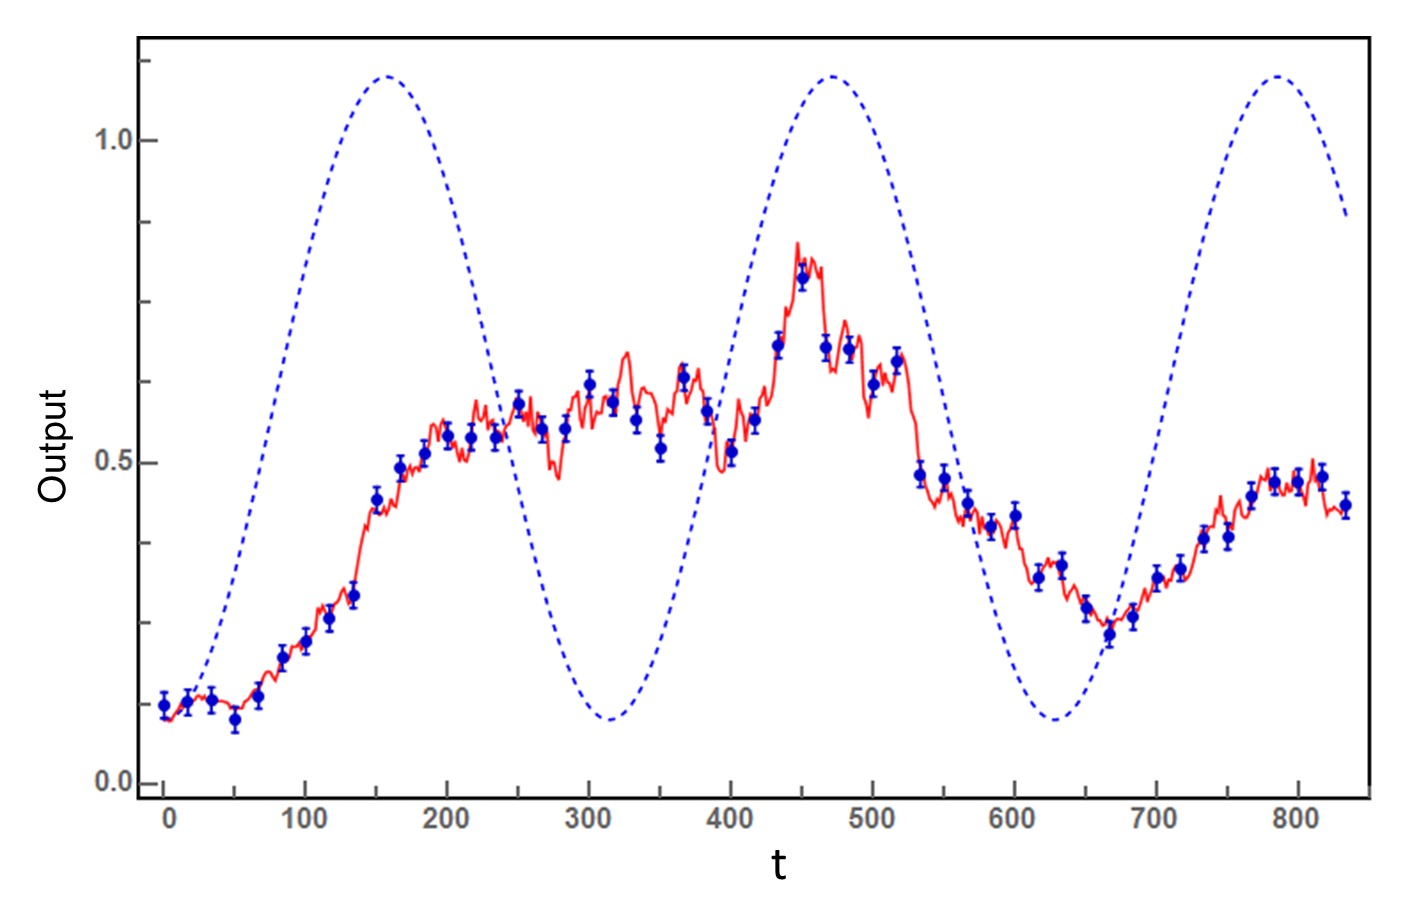
\includegraphics[width=0.4\textwidth]{Figs/FigRainData.png}
    \caption{\label{fig:rain_data_S}Rain input (dashed), system realization (solid line) and synthetic experimental data. The system output and the observed data were generated using $K=200$ and $\gamma = 0.2$.}
\end{figure}

\begin{figure}[htb!]
    \centering
    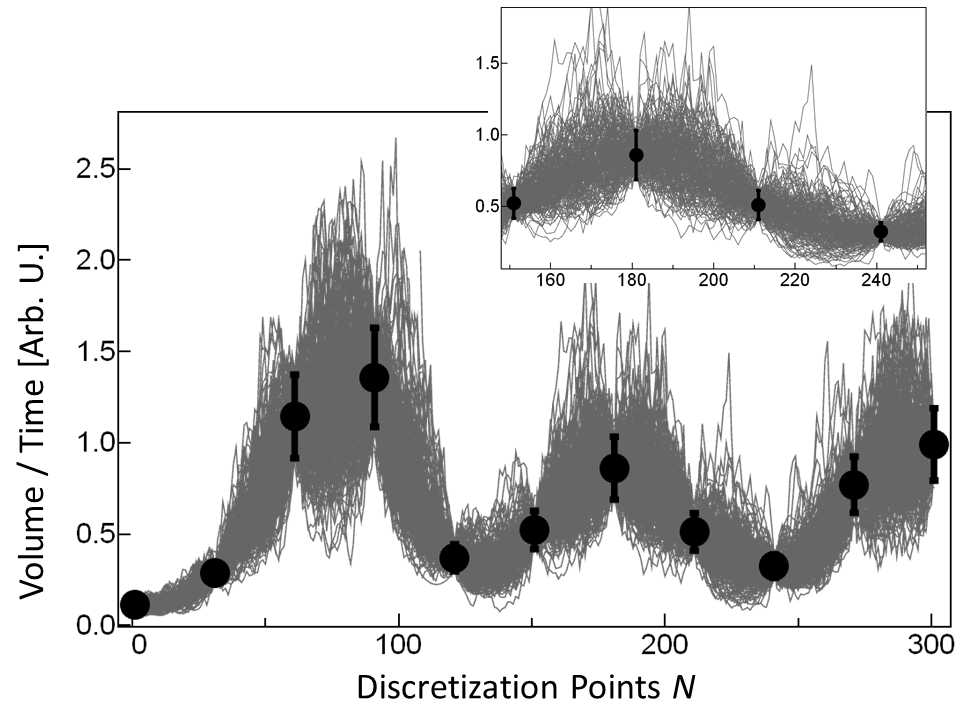
\includegraphics[width=0.5\textwidth]{Figs/FigSpaghetti.png}
    \caption{Simulated system realizations and synthetic experimental data obtained assuming a simple sinusoidal model for the rain input. In the inset one may appreciate the different dynamics of the heavy data-point beads and the light staging beads.}
    \label{fig:spaghetti}
\end{figure}

\begin{figure}[htb!]
    \centering
    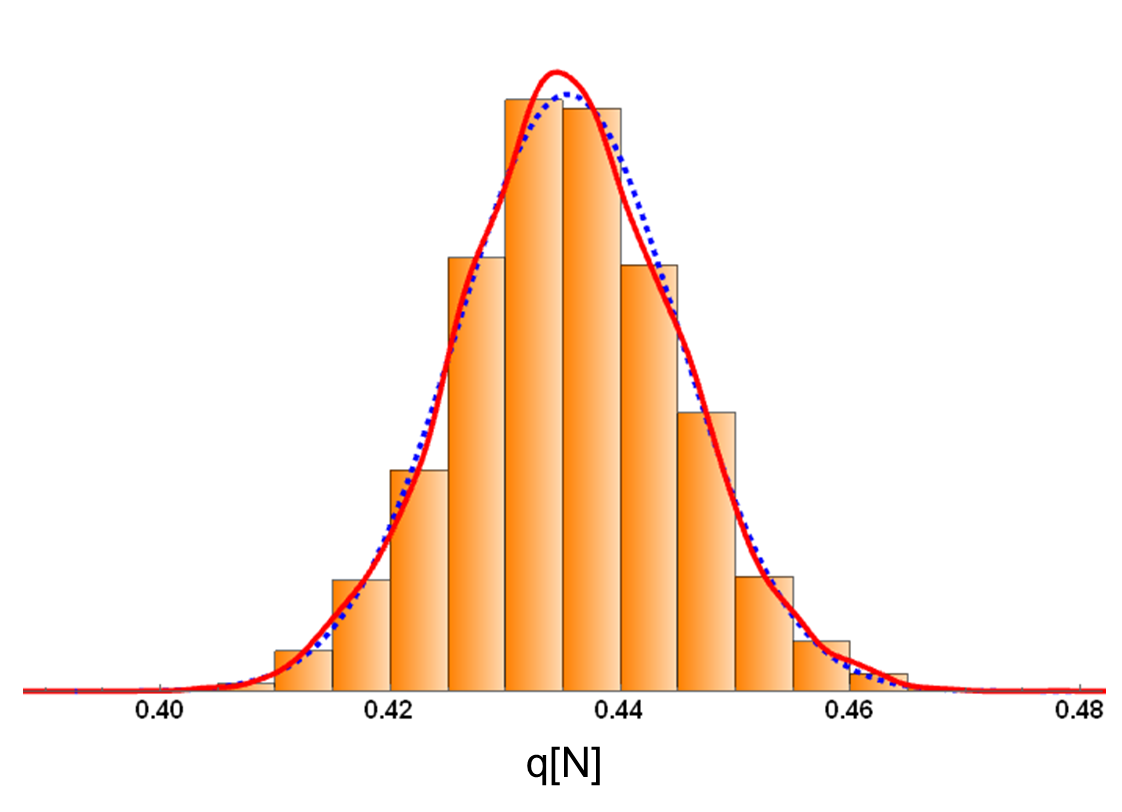
\includegraphics[width=0.3\textwidth]{Figs/FigFinalState.png}
    \caption{PDF for the system final state expressed via the coordinate set $\left\{ q_N \right\}$. The dashed curve represents a normal distribution with the same mean and variance. The final state is basically normally distributed.}
    \label{fig:final_state}
\end{figure}

\begin{figure}[htb!]
    \centering
    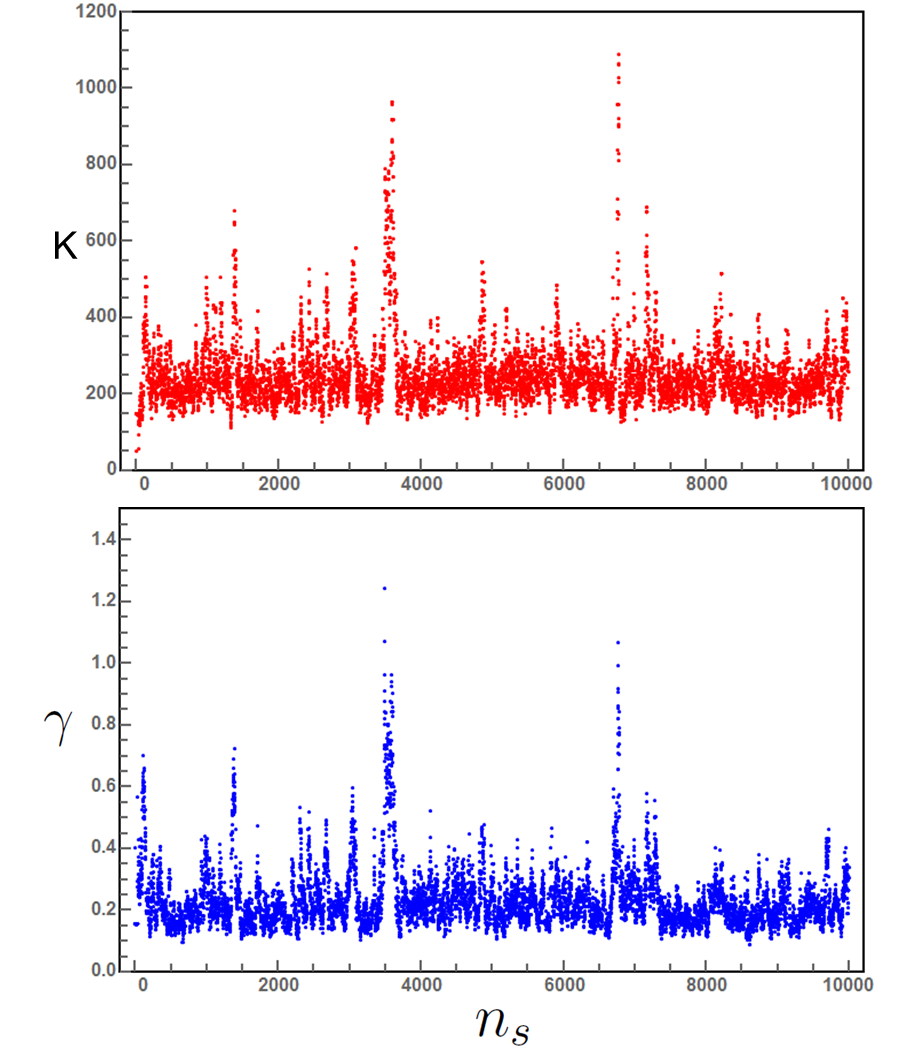
\includegraphics[width=0.4\textwidth]{Figs/FigChains.png}
    \caption{Markov chains for the two parameters $K$ (top) and $\gamma$ (bottom).}
    \label{fig:chains}
\end{figure}

\begin{figure}[htb!]
    \centering
    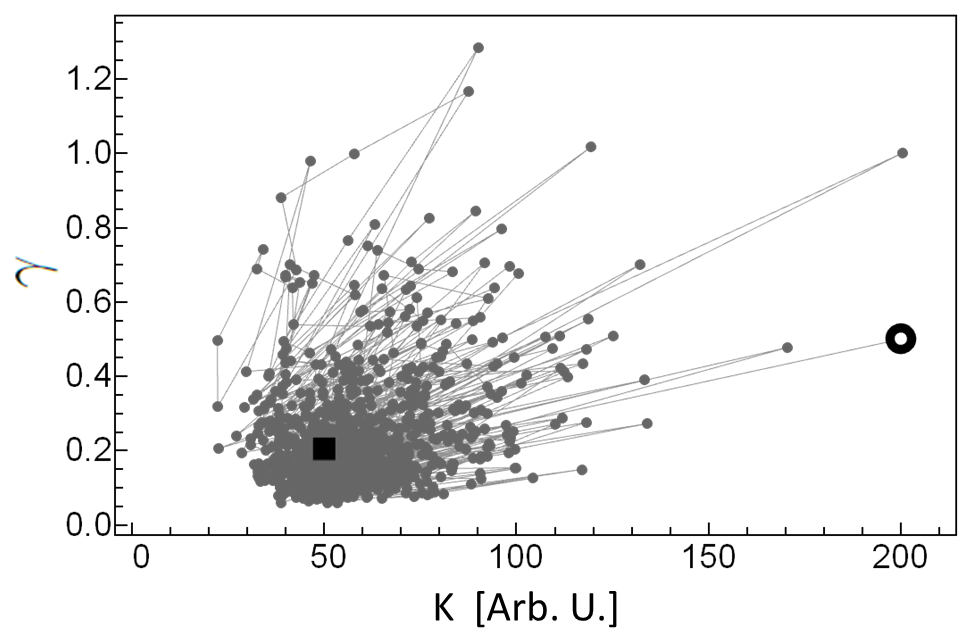
\includegraphics[width=0.5\textwidth]{Figs/FigPhaseSpaceEvol.png}
    \caption{System dynamics in the phase space $K-\gamma$. The green dot is the initial state, the red dot is the final state, the yellow dots are the last 50 states of the HMC chain, and the orange square corresponds to the true parameter values used to generate the data.}
    \label{fig:phase_space_evol}
\end{figure}

\begin{figure}[htb!]
    \centering
    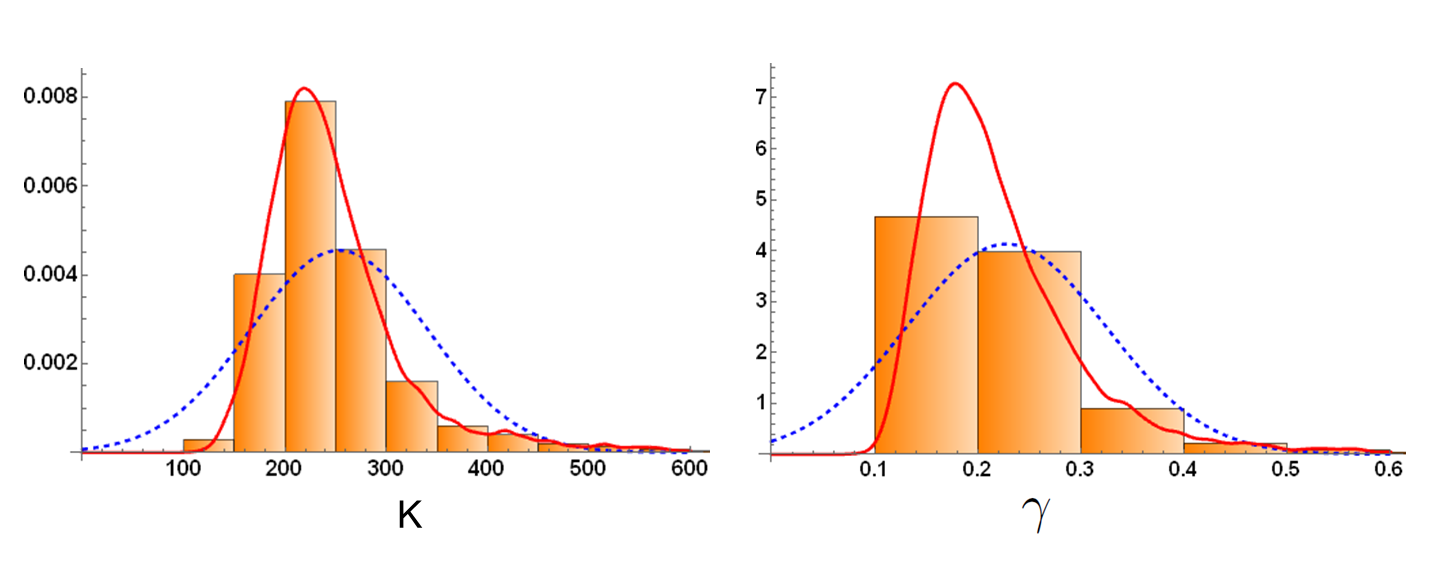
\includegraphics[width=0.5\textwidth]{Figs/FigKg.png}
    \caption{PDF for the parameters $K$ (left) and $\gamma$ (right). The true values used to generate the data are $K=200$ and $\gamma = 0.2$. The initial values used in the simulations were $K=50$ and $\gamma = 0.4$.}
    \label{fig:K_distr}
\end{figure}

\subsection{Sample subsection}

Lorem ipsum dolor sit amet, consectetur adipiscing elit, sed do eiusmod tempor incididunt ut labore et dolore magna aliqua. Ut enim ad minim veniam, quis nostrud exercitation ullamco laboris nisi ut aliquip ex ea commodo consequat. Duis aute irure dolor in reprehenderit in voluptate velit esse cillum dolore eu fugiat nulla pariatur. Excepteur sint occaecat cupidatat non proident, sunt in culpa qui officia deserunt mollit anim id est laborum.

\subsubsection{Sample subsubsection}

Lorem ipsum dolor sit amet, consectetur adipiscing elit, sed do eiusmod tempor incididunt ut labore et dolore magna aliqua. Ut enim ad minim veniam, quis nostrud exercitation ullamco laboris nisi ut aliquip ex ea commodo consequat. Duis aute irure dolor in reprehenderit in voluptate velit esse cillum dolore eu fugiat nulla pariatur. Excepteur sint occaecat cupidatat non proident, sunt in culpa qui officia deserunt mollit anim id est laborum.

\begin{figure}[htb!]
 \centering
 
\includegraphics{lion.png}
 \caption{\label{figureone}This is sample picture -- ShareLaTeX lion. }
\end{figure}


\subsection{Simplified coding and extra features for tables}
The basic coding format can be simplified using extra commands provided in
the \verb"iopart" class file. The commands up to and including
the start of the tabular environment
can be replaced by
\small\begin{verbatim}
\Table{\label{label}Table caption}
\end{verbatim}\normalsize
this also activates the definitions within \verb"\lineup".
The final three lines can also be reduced to \verb"\endTable" or
\verb"\endtab". Similarly for a table which does not fit in when indented
\verb"\fulltable{\label{label}caption}" \dots\ \verb"\endfulltable" or \verb"\endtab"
can be used. \LaTeX\ optional positional parameters can, if desired, be added after
\verb"\Table{\label{label}caption}" and \verb"\fulltable{\label{label}caption}".


\verb"\centre{#1}{#2}" can be used to centre a heading
\verb"#2" over \verb"#1"
columns and \verb"\crule{#1}" puts a rule across
\verb"#1" columns. A negative
space \verb"\ns" is usually useful to reduce the space between a centred
heading and a centred rule. \verb"\ns" should occur immediately after the
\verb"\\" of the row containing the centred heading (see code for
\tref{tabl1}). A small space can be
inserted between rows of the table
with \verb"\ms" and a half line space with \verb"\bs"
(both must follow a \verb"\\" but should not have a
\verb"\\" following them).

\Table{\label{tabl1}A table with headings spanning two columns and containing notes.
To improve the
visual effect a negative skip ($\backslash${\tt ns})
has been put in between the lines of the
headings. Commands set-up by $\backslash${\tt lineup} are used to aid
alignment in columns. $\backslash${\tt lineup} is defined within
the $\backslash${\tt Table} definition.}
\br
&&&\centre{2}{Separation energies}\\
\ns
&Thickness&&\crule{2}\\
Nucleus&(mg\,cm$^{-2}$)&Composition&$\gamma$, n (MeV)&$\gamma$, 2n (MeV)\\
\mr
$^{181}$Ta&$19.3\0\pm 0.1^{\rm a}$&Natural&7.6&14.2\\
$^{208}$Pb&$\03.8\0\pm 0.8^{\rm b}$&99\%\ enriched&7.4&14.1\\
$^{209}$Bi&$\02.86\pm 0.01^{\rm b}$&Natural&7.5&14.4\\
\br
\end{tabular}
\item[] $^{\rm a}$ Self-supporting.
\item[] $^{\rm b}$ Deposited over Al backing.
\end{indented}
\end{table}

\section*{References}
\bibliographystyle{unsrt}
\bibliography{refs}

%\section*{References}
%\begin{thebibliography}{10}
%\bibitem{ref1} J.~Doe, Article name, \textit{Phys. Rev. Lett.}
%\bibitem{ref2} J.~Doe, J. Smith, Other article name, \textit{Phys. Rev. Lett.}
%\bibitem{web} \href{http://www.google.pl}{www.google.pl}
%\end{thebibliography}

\end{document}

